\documentclass[tikz,border=8pt]{standalone}
% Shared look for every TikZ diagram. Load with % Shared look for every TikZ diagram. Load with % Shared look for every TikZ diagram. Load with \input{../../tools/tikz-style.tex}
\usepackage[T1]{fontenc}
\usepackage{lmodern}
\renewcommand{\sfdefault}{lmr}  % diagrams use the same serif as the text
\usetikzlibrary{arrows.meta, positioning, shapes.geometric, calc, fit, backgrounds}
\definecolor{cblue}{HTML}{4C78A8}
\definecolor{corange}{HTML}{F58518}
\definecolor{cgreen}{HTML}{54A24B}
\definecolor{cred}{HTML}{E45756}
\definecolor{cpurple}{HTML}{B279A2}
\definecolor{cgrey}{HTML}{6B6B6B}
\tikzset{
  every picture/.style={font=\sffamily, line width=1.2pt},
  box/.style={draw=#1, fill=#1!12, rounded corners=4pt, align=center, inner sep=7pt, minimum height=1.1cm},
  box/.default=cgrey,
  arrow/.style={-{Stealth[length=3mm]}, draw=cgrey, line width=1.4pt},
  title/.style={font=\sffamily\bfseries\Large},
  note/.style={font=\sffamily\small, text=cgrey, align=center},
}
\AtBeginDocument{\hyphenpenalty=10000 \exhyphenpenalty=10000}

\usepackage[T1]{fontenc}
\usepackage{lmodern}
\renewcommand{\sfdefault}{lmr}  % diagrams use the same serif as the text
\usetikzlibrary{arrows.meta, positioning, shapes.geometric, calc, fit, backgrounds}
\definecolor{cblue}{HTML}{4C78A8}
\definecolor{corange}{HTML}{F58518}
\definecolor{cgreen}{HTML}{54A24B}
\definecolor{cred}{HTML}{E45756}
\definecolor{cpurple}{HTML}{B279A2}
\definecolor{cgrey}{HTML}{6B6B6B}
\tikzset{
  every picture/.style={font=\sffamily, line width=1.2pt},
  box/.style={draw=#1, fill=#1!12, rounded corners=4pt, align=center, inner sep=7pt, minimum height=1.1cm},
  box/.default=cgrey,
  arrow/.style={-{Stealth[length=3mm]}, draw=cgrey, line width=1.4pt},
  title/.style={font=\sffamily\bfseries\Large},
  note/.style={font=\sffamily\small, text=cgrey, align=center},
}
\AtBeginDocument{\hyphenpenalty=10000 \exhyphenpenalty=10000}

\usepackage[T1]{fontenc}
\usepackage{lmodern}
\renewcommand{\sfdefault}{lmr}  % diagrams use the same serif as the text
\usetikzlibrary{arrows.meta, positioning, shapes.geometric, calc, fit, backgrounds}
\definecolor{cblue}{HTML}{4C78A8}
\definecolor{corange}{HTML}{F58518}
\definecolor{cgreen}{HTML}{54A24B}
\definecolor{cred}{HTML}{E45756}
\definecolor{cpurple}{HTML}{B279A2}
\definecolor{cgrey}{HTML}{6B6B6B}
\tikzset{
  every picture/.style={font=\sffamily, line width=1.2pt},
  box/.style={draw=#1, fill=#1!12, rounded corners=4pt, align=center, inner sep=7pt, minimum height=1.1cm},
  box/.default=cgrey,
  arrow/.style={-{Stealth[length=3mm]}, draw=cgrey, line width=1.4pt},
  title/.style={font=\sffamily\bfseries\Large},
  note/.style={font=\sffamily\small, text=cgrey, align=center},
}
\AtBeginDocument{\hyphenpenalty=10000 \exhyphenpenalty=10000}

\begin{document}
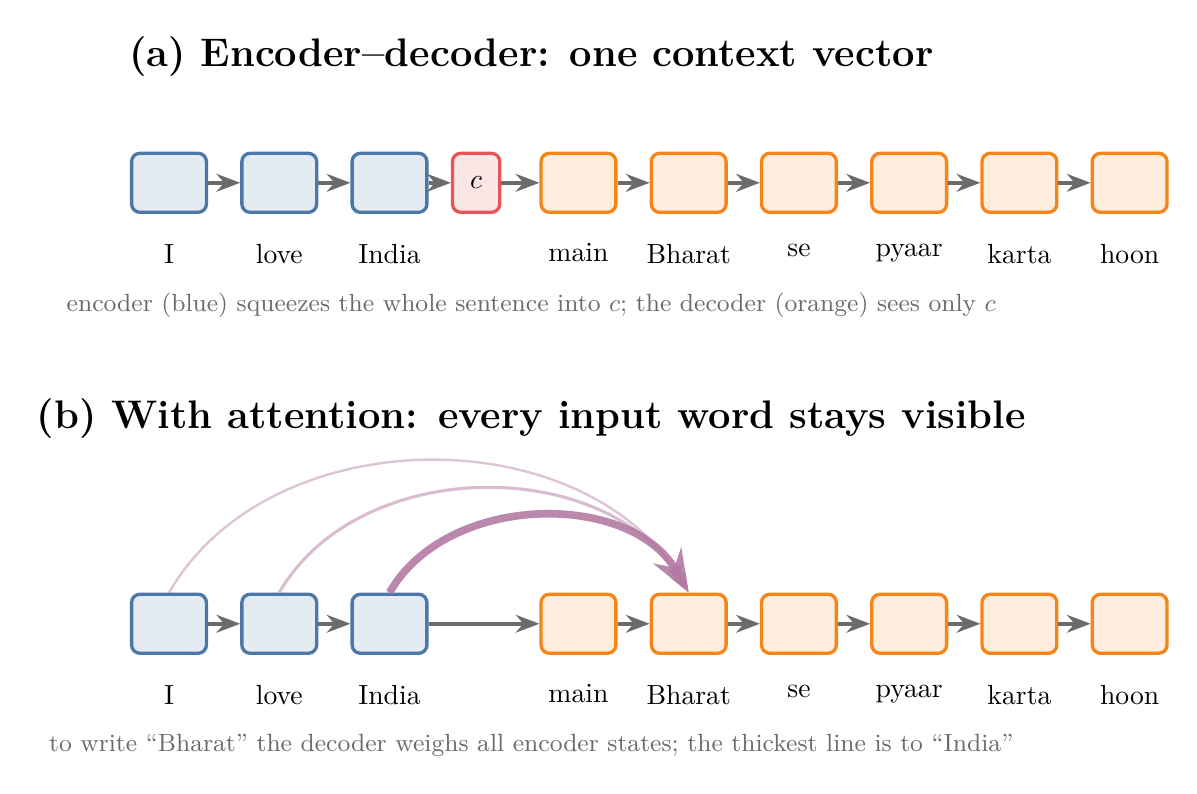
\begin{tikzpicture}[cell/.style={draw=#1, fill=#1!15, minimum width=0.95cm, minimum height=0.75cm, rounded corners=3pt},
  word/.style={font=\sffamily}]
  % (a) plain encoder-decoder
  \node[title] at (6.0, 1.6) {(a) Encoder--decoder: one context vector};
  \foreach \w [count=\i] in {I, love, India} {
    \node[cell=cblue] (e\i) at (1.4*\i, 0) {};
    \node[word, below=0.25cm of e\i] {\w};
  }
  \draw[arrow] (e1) -- (e2); \draw[arrow] (e2) -- (e3);
  \node[cell=cred, minimum width=0.6cm] (c) at (5.3, 0) {$c$};
  \draw[arrow] (e3) -- (c);
  \foreach \w [count=\i] in {main, Bharat, se, pyaar, karta, hoon} {
    \node[cell=corange] (d\i) at (5.2+1.4*\i, 0) {};
    \node[word, below=0.25cm of d\i] {\w};
  }
  \draw[arrow] (c) -- (d1); \draw[arrow] (d1) -- (d2); \draw[arrow] (d2) -- (d3); \draw[arrow] (d3) -- (d4); \draw[arrow] (d4) -- (d5); \draw[arrow] (d5) -- (d6);
  \node[note] at (6.0, -1.55) {encoder (blue) squeezes the whole sentence into $c$; the decoder (orange) sees only $c$};
  % (b) attention
  \begin{scope}[yshift=-5.6cm]
  \node[title] at (6.0, 2.6) {(b) With attention: every input word stays visible};
  \foreach \w [count=\i] in {I, love, India} {
    \node[cell=cblue] (f\i) at (1.4*\i, 0) {};
    \node[word, below=0.25cm of f\i] {\w};
  }
  \draw[arrow] (f1) -- (f2); \draw[arrow] (f2) -- (f3);
  \foreach \w [count=\i] in {main, Bharat, se, pyaar, karta, hoon} {
    \node[cell=corange] (g\i) at (5.2+1.4*\i, 0) {};
    \node[word, below=0.25cm of g\i] {\w};
  }
  \draw[arrow] (f3) -- (g1); \draw[arrow] (g1) -- (g2); \draw[arrow] (g2) -- (g3); \draw[arrow] (g3) -- (g4); \draw[arrow] (g4) -- (g5); \draw[arrow] (g5) -- (g6);
  \foreach \i/\o in {1/0.15, 2/0.25, 3/0.9} \draw[cpurple, line width=0.5pt+2.5pt*\o, opacity=0.35+0.6*\o, -{Stealth}] (f\i.north) to[out=60, in=120] (g2.north);
  \node[note] at (6.0, -1.55) {to write ``Bharat'' the decoder weighs all encoder states; the thickest line is to ``India''};
  \end{scope}
\end{tikzpicture}
\end{document}
